\documentclass{article}
\usepackage[french]{babel}
\usepackage[utf8]{inputenc}
\usepackage{graphicx}
\usepackage{dejavu}
\renewcommand*\familydefault{\sfdefault} %% Only if the base font of the document is to be sans serif
\usepackage[T1]{fontenc}

\usepackage{geometry}
\geometry{a4paper,headheight=16pt,tmargin=25mm,
          bmargin=25mm,lmargin=20mm,rmargin=20mm}

\usepackage{fancyhdr}
\usepackage{lastpage}

\usepackage{hyperref}
\usepackage{array}
\usepackage{color}
 
\pagestyle{fancy}
\fancyhf{}
\lhead{\footnotesize Première STI2D\\Tronc commun}
\chead{\large Simulation d’une loi de base sur les puissances}
\lfoot{Lycée Blaise Pascal}
\rfoot{\thepage/\pageref{LastPage}}

\renewcommand{\headrulewidth}{1pt}
\renewcommand{\footrulewidth}{1pt}

\begin{document}
\begin{center}
%	\begin{flushright}
%		\begin{Form}
%			\TextField[name=nom,width=10em,default=Nom]{Nom:}\\
%			\TextField[name=prenom,width=10em,default=Prénom]{Prénom:}\\
%			\TextField[name=classe,width=10em,default=Classe]{Classe:}\\
%		\end{Form}
%	\end{flushright}

	\vspace{1em}
	\Large
	\textbf{Objectif:} Retrouver par simulation la loi d’additivité des puissances. Prendre en main le logiciel ISIS/Proteus.
\end{center}

\vspace{2em}
\begin{minipage}[b]{0.68\linewidth}
Jacky souhaite changer les phares de sa 206 GTI tuning.
Les deux lampes bleues qu'il a acheté sont de 90W alors que celles d'origine sont de 60W.

Jacky compte bricoler le faisceau électrique de sa voiture pour mettre les ampoules en série à la place du montage parallèle d'origine.
Il pense ainsi résoudre le problème, car comme le même courant traverse les deux ampoules, la puissance devrait être divisée par 2.\\

\end{minipage}
\hfill
\begin{minipage}[b]{0.28\linewidth}
	\centering
	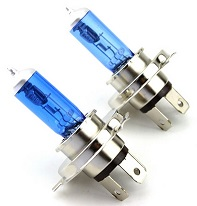
\includegraphics[width=.8\linewidth]{./figures/phare1.png}
\end{minipage}

Jacky se trompe, nous allons lui expliquer pourquoi dans cette activité.
	

\vspace{2em}
\textbf{Production attendue:} 
Vous rédigerez un compte rendu de simulation sous forme d’un diaporama. Il devra préciser :
\begin{itemize}
	\item les réponses aux questions préliminaires
	\item les schémas électriques des 2 simulations
	\item les mesures de toutes les tensions et intensités de ces schémas
	\item les calculs de puissance découlant de ces mesures
	\item les conclusions que vous pouvez tirer des mesures et calculs :
		\begin{itemize}
			\item sur le fonctionnement correct ou non du montage en parallèle
			\item sur le fonctionnement correct ou non du montage en série
			\item sur l’équation reliant la puissance globale fournie par la batterie et la puissance consommée par les lampes, quel que soit le type de montage.
		\end{itemize}
	\item les réponses aux questions complémentaires de la partie 2.3 si vous avez le temps de les traiter.
\end{itemize}

\vspace{1em}

\section{Questions préliminaires}
\begin{minipage}[b]{0.48\linewidth}
\paragraph{Q1:}
D’après l’étiquette de batterie de voiture ci-contre, quelle tension est disponible dans le véhicule pour faire fonctionner l’éclairage (entre autres) ?
	\vspace{1.5em}
\end{minipage}
\hfill
\begin{minipage}[b]{0.48\linewidth}
	\centering
	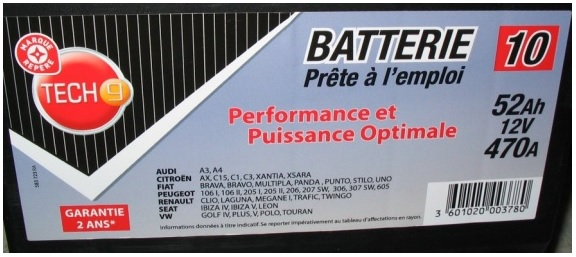
\includegraphics[width=.8\linewidth]{./figures/batterie1.png}
\end{minipage}

\vspace{1em}

\begin{minipage}[b]{0.68\linewidth}
\paragraph{Q2:}
D’après la boite d’ampoule ci-contre, à quelle tension doivent être alimentées des ampoules de phare pour éclairer correctement ?
	\vspace{5em}
\end{minipage}
\hfill
\begin{minipage}[b]{0.28\linewidth}
	\centering
	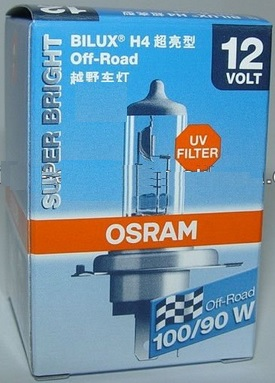
\includegraphics[width=.8\linewidth]{./figures/phare2.png}
\end{minipage}

\newpage

En électricité, la puissance consommée par un appareil ou un composant se calcule de différentes façons
suivant le type d’alimentation électrique utilisé.\\

\begin{center}
	\begin{tabular}{|c|c|}
		\hline
		Type de tension électrique & Formule à appliquer \\
		\hline
		\hline
		Continue & $P = U \times I$\\
		\hline
		Alternatif simple (monophasé) & $P = U \times I \times cos(\varphi)$ \\
		\hline
		Alternatif triphasé & $P = \sqrt{3} \times U \times I \times cos(\varphi)$\\
	
		\hline
	\end{tabular}

	avec $U$ la tension aux bornes de l’élément considéré, $I$ l’intensité du courant qui le traverse
	et $\varphi$ le déphasage entre $U$ et $I$.
\end{center}

\vspace{1em}
\paragraph{Q3:} Dans le cas qui nous intéresse aujourd’hui, quelle formule va-t-on devoir utiliser ?

\paragraph{Q4:} Rappeler les symboles électriques, grandeurs physiques mesurée, les unités, ainsi que les types de montage du voltmètre et de l'ampèremètre.

\section{Simulations avec ISIS/Proteus}
Pour effectuer le travail ci-dessous, vous disposez du fichier ressource sur Proteus disponible dans le répertoire de l’activité.

\paragraph{Q5:} À partir du fichier de simulation Proteus \og{}simulation éclairage voiture –ELEVE.DSN\fg{} 
fourni dans le répertoire de l’activité, vous devez réaliser 2 simulations prouvant :
\begin{itemize}
	\item que seul le montage d’origine permet un fonctionnement correct de l’éclairage
	\item que la formule de calcul de la puissance globale consommée est la même quel que soit le type de montage.
\end{itemize}

\section{Questions complémentaires}
\paragraph{Q6:} Outre le fait que le montage en série ne fonctionne pas correctement dans ce cas, à votre avis, quel problème sécuritaire supplémentaire pose-t-il ?
\paragraph{Q7:} Déterminer ou vérifier par simulation la tension de batterie qui serait nécessaire pour que le montage en série fonctionne correctement. 
La loi sur les puissances déterminée à la question \textbf{Q5} est- elle toujours vérifiée ?


\end{document}
